\documentclass[pdftex, 11pt, a4paper]{article}
\usepackage[pdftex]{graphicx}
\usepackage[utf8]{inputenc}
\usepackage{appendix}
\usepackage{rotating}
\usepackage{pdflscape}
\usepackage[breaklinks=true]{hyperref}
\usepackage{listings}
\usepackage{nomencl}
\usepackage[a4paper]{geometry}
\usepackage{tabularx}
\usepackage{longtable}
\usepackage{listings}
\usepackage{fancyvrb}
\usepackage{color}
\usepackage[style=ieee]{biblatex}
\usepackage{mathtools}

\bibliography{main}

\title{Cryptography Assignment}
\author{
    Thomas A. Grainger \\
    Department of Electronics and Computer Science\\
    University of Southampton\\
}
\date{\today}

\lstset{
    basicstyle=\footnotesize,
    frame=single,
    numbers=left,
    breaklines=true,
    caption=\lstname
}

\RecustomVerbatimCommand{\VerbatimInput}{VerbatimInput}{
    fontsize=\footnotesize,
    framesep=2em, % separation between frame and text
}

\begin{document}
\maketitle

\begin{abstract}
This report aims to solve a series of challenges set by~\textcite{instructions},
aiming for both thoroughness of methodology and accuracy of solution. The
cryptographic decryption challenges demonstrate the use of Python as a useful
tool to create automated cipher decryption systems.
\end{abstract}

\tableofcontents
\pagebreak
\section{Linear feedback shift register}
Part one involves the decryption of what appears to be a block of hexadecimal encoded data.  It is given that the second encryption scheme is an LFSR and a crib of ``Ur'' is divulged.  There were two main observations made initially: a repeating pattern of high bits every 32 bits was present and that the ciphertext was presented as a bitmap.  The unusual delivery method hinted that steganographic techniques could have been used however, after some analysis, no embedded information was revealed.

\subsection{Compromising LFSR encryption}
An LFSR of degree 5 will repeat every 31 bits, however, referring back to the first observation of the ciphertext that there is a pattern of high bits repeating every 32 bits. This observation clearly contradicts the hint that the second encryption stage uses an LFSR of degree 5 and indicates that the text was encrypted using a 32 bit repeating key.

A program, shown in appendix~\ref{last-byte}, was created to determine the repeating 32 bit key using brute force. The brute force was made feasible using the assumption that the first 3 bytes of the repeating key were from a valid 31 bit LFSR key-stream and that the mid-stage ciphertext would only contain printable characters. This resulted in only one valid solution.

\subsection{Compromising a non-standard LFSR encryption implementation}
The mid-stage ciphertext, shown in appendix~\ref{last-byte-out}, shows signs consistent with the use of a mono-alphabetic substitution cipher: the use of repeated three letter words ``pna'' and ``gur'' potentially indicating ``and'' and ``the''; long repeated words ``Ubjrire'' and apparant use of English punctuation such as commas and capital letters after full-stops.

In fact, this ciphertext is a mono-alphabetic substitution cipher and as such the remaining ciphertext could be decrypted using techniques as discussed in section~\ref{mono}.  The final solution is shown in appendix~\ref{q1-solution}.

\section{Hamming codes and generator polynomials}
\subsection{Part a}
The properties of generator polynomials can be used to determine if a polynomial
is a generator polynomial.  A generator polynomial is also known as a primitive
polynomial and ``primitive polynomials are also irreducible
polynomials''~\cite{wolfram-primative}.  As such any polynomial that can be
factorized modulus 2 is not a generator polynomial.

\begin{description}
    \item[$f1(x) = x^6 + x^3 + x^2 + x + 1$] is reducible because $f1(x) = (x^2+x+1)(x^4+x^3+1)$.
    \item[$f2(x) = x^6 + x^5 + x^4 + x^3 + 1$] is reducible because $f2(x) = (x^2+x+1)(x^4+x+1)$.
    \item[$f3(x) = x^6 + x^5 + x$] is reducible because $f3(x) = x(x^5 + x^4 + 1)$.
    \item[$f4(x) = x^6 + x^5 +x^4 + x^2 +x + 1$] is reducible because $f4(x) = (x^2+x+1)(x+1)^4$.
    \item[$f5(x) = x^6 + x + 1$] is a generator polynomial by elimination.
\end{description}

These justifications can be tested using the two argument version of the
``hammgen'' function from GNU Octave~\cite{hammgen-octave}, also a function
available in MATLAB~\cite{hammgen-matlab}. Using this function it is possible to
determine if a polynomial is a generator polynomial of a hamming code or not:
when a non-generator polynomial is given as the function's second argument an
exception is raised.  A program to test all of the given polynomials, shown in
appendix~\ref{hammgen}, concluded that $f5(x)$ is the only generator polynomial
out of the given functions.

\subsection{Part b}
Using the ``hammgen'' function from GNU Octave~\cite{hammgen-octave} a program,
shown in appendix~\ref{hammgen-hg}, was created to output the parity check,
H\label{parity-check}, and generator, G, matrices for $f5(x)$.
See appendix~\ref{h-matrix} for the H matrix and appendix~\ref{g-matrix} for the
G matrix.

\subsection{Part c}
Using the parity check matrix, H, from section~\ref{parity-check} it is possible
to determine if a message is a valid code word: ``In coding theory, a
parity-check matrix of a linear block code C is a generator matrix of the dual
code. As such, a codeword c is in C if and only if the matrix-vector product
$Hc^t = 0$''~\cite{check-matrix}. A program, included in
appendix~\ref{check-matrix}, was written to determine that the valid code words
are m1 and m2.

\section{Mono-alphabetic substitution}\label{mono}
In this challenge, another decryption challenge, the requirement is to decrypt a
block of text included in appendix~\ref{q3-cyphertext}. This time there is no
hint provided.

The clue that the cypher-text is the result of mono-alphabetic
substitution is the use of repeated words such as ``uli'' and ``blf''
potentially indicating the English three letter words ``and'' and ``the''.
A program, included in appendix~\ref{break-simplesub}, based on work by
\textcite{stochastic-searching} was used to successfully break the cypher.
The solution is included in appendix~\ref{q3-solution}.
While a frequency analysis would also be useful for solving these sorts of cyphers in
general, this was not used because of the success of the automated simple
substitution breaking program.

\section{The miss-application of RC4 and CRC32 in WEP}\label{conclusions}

\subsection{Part a}
\subsubsection{What is WEP}
The Wired Equivalent Privacy (WEP) security algorithm was released with the original 802.11 standard in 1999\cite{802.11}. This system was designed to be be responsible for both authentication (access control), encryption (confidentiality) and data integrity in Wi-Fi networks.

The name comes from the intention that it would provide the same level of security as a wired connection, however according to \textcite{intercepting-wifi}, ``despite employing the well-known and believed-secure RC4 cipher, WEP contains several major security flaws.''.  The answer to this question aims to detain the cryptographic tools used and the flaws introduced by their miss-application.

\subsubsection{Rivest Cipher 4}
The Rivest Cipher 4 (RC4) encryption algorithm from RSA Data Security is a stream cipher, these ciphers simulate the operation of a one-time-pad using a pseudo random number generator (PRNG) seeded from a key\cite{otp-faq}. When encrypting binary data, each bit of the plain-text is XORed with a bit of the generated key-stream. To decrypt the system the same random cipher-stream is generated using the same key, or seed to the RC4 cipher.

One major disadvantage of one time pad, or stream cipher, systems is that if two messages are encrypted with the same key the ciphertexts of those messages can be subjected to cryptanalysis.  The reason for this, shown in equation~\ref{eq:xor} or graphically in equation~\ref{eq:img-xor}, is that the cipher stream can be eliminated by calculating the xor of the two related ciphertexts. An even worse situation is when a message using the same cipher-stream as a previous message with one of those messages containing known plain-text, with this key information for future messages can be derived.

\begin{subequations}
    \begin{align}
        P_1 \oplus KS = C_1,\\
        P_2 \oplus KS = C_2,\\
        C_1 \oplus C_2 = P_1 \oplus P_2\label{eq:xor}
    \end{align}
\end{subequations}

\begin{figure}[htb]
\begin{subequations}
    \begin{align}
        \overbrace{
\includegraphics[height=8ex]{img/sendcash1}}^{P_1} \oplus \overbrace{
\includegraphics[height=8ex]{img/key1}}^{KS} = \overbrace{
\includegraphics[height=8ex]{img/sendcashe}}^{C_1},\\
        \overbrace{
\includegraphics[height=8ex]{img/smiley}}^{P_2}    \oplus \overbrace{
\includegraphics[height=8ex]{img/key1}}^{KS} =\overbrace{
\includegraphics[height=8ex]{img/smileye}}^{C_2},\\
        \overbrace{
\includegraphics[height=8ex]{img/sendcashe}}^{C_1} \oplus \overbrace{
\includegraphics[height=8ex]{img/smileye}}^{C_2} = \overbrace{
\includegraphics[height=8ex]{img/smicash1}}^{P_1 \oplus P_2}\label{eq:img-xor}
    \end{align}
\end{subequations}
\caption{Graphical representation of why reusing a keystream is dangerous cryptographically: It is clear that some plain-text can be determined from this method (source \protect\cite{stream-reuse})}
\end{figure}

\subsubsection{Application of RC4 in WEP}
WEP uses a 40-bit shared key to initialize the same RC4 state for all authenticated stations, the reason for using only 40-bits was to comply with US restrictions on exporting cryptography technology\cite{wep-evolution}.

RC4 is a stream-cipher and so any missing data causes a misalignment with the key-stream this is a major problem in Wi-Fi, or any Ethernet based protocol, where frames are expected to be lost.
To avoid misalignment problems the RC4 stream is restarted each frame. This is not the intended use of a stream cipher therefore stream reuse must be prevented. In WEP this is done using a public random 24-bit Initialization Vector (IV)~\label{p:iv}.  The vast majority of the flaws of WEP are due to this misuse of a stream-cipher. This process is shown in figure~\ref{fig:wepop}.

\subsubsection{Application of CRC32 in WEP}
Every frame includes an Integrity Check Value (ICV) which is the Cyclic Redundancy Check (CRC-32) hash of the plain-text appended to the plain-text prior to encryption the receiver then re-computes the CRC-32 hash of the message after decryption and if it does not match the frame is dropped. This process is also shown in figure~\ref{fig:wepop}.

\begin{figure}[htb]
\center
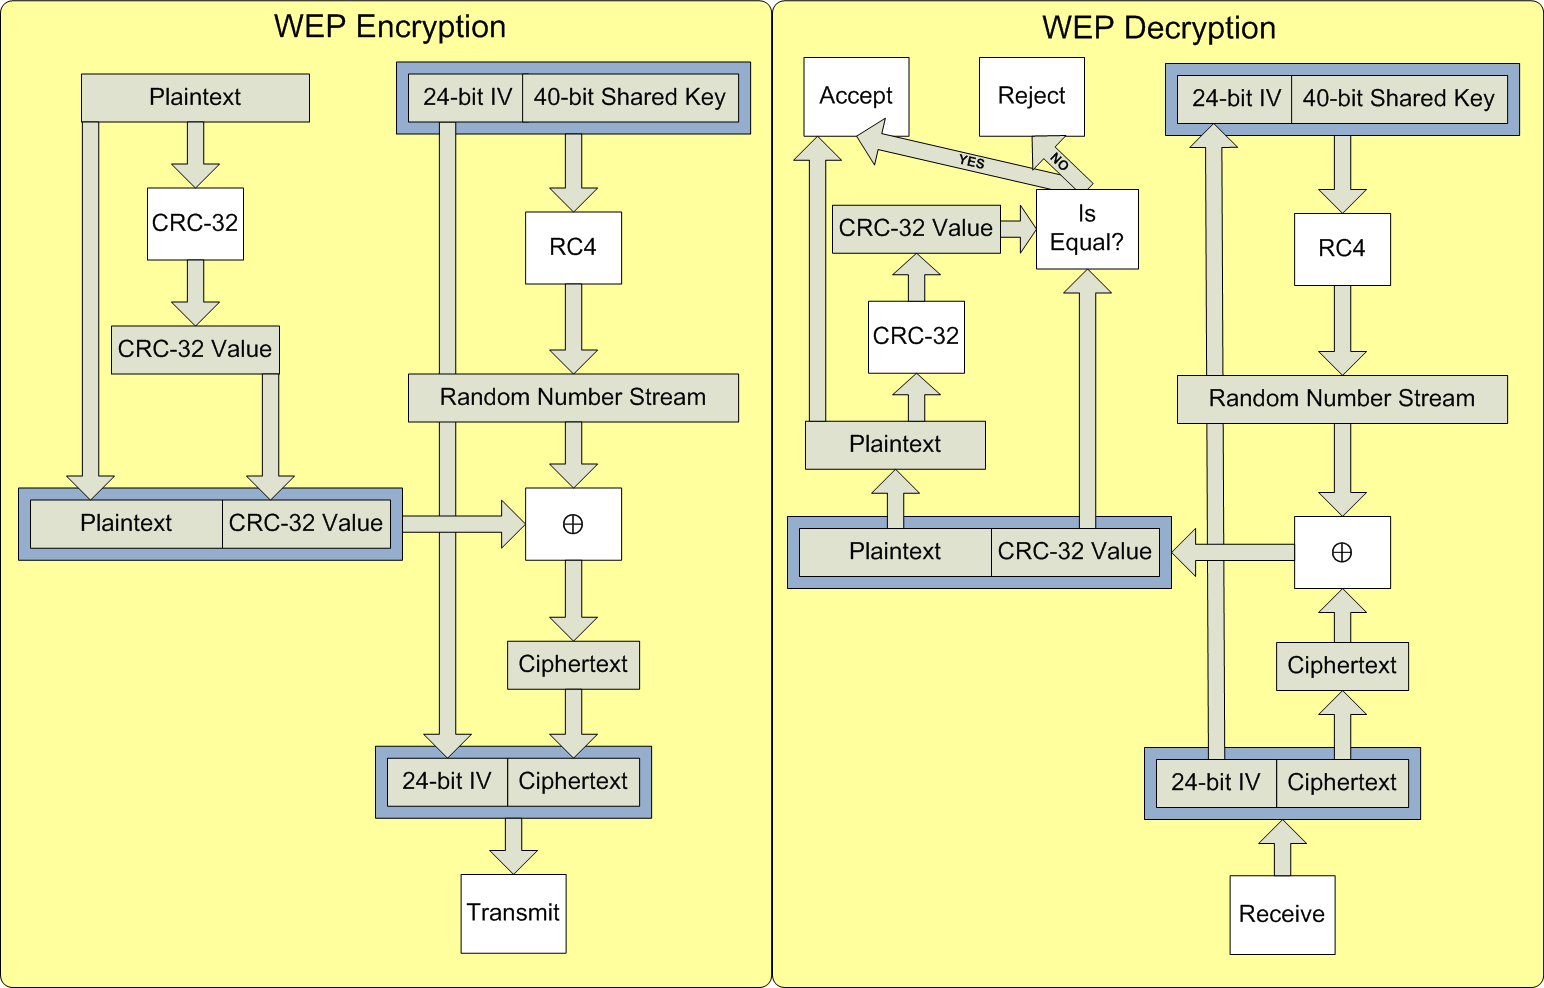
\includegraphics[width=0.9\linewidth]{img/wepOperation}\label{fig:wepop}
\caption{Diagram showing the encryption and decryption operations of WEP (source \protect\cite{wep-evolution})}
\end{figure}

\subsubsection{Flaws}

\paragraph{Integrity Check Value}
The CRC used in the ICV is a poor cryptographic hash because it is a linear function of the message. Check-sum algorithms are ``unsuitable as cryptographic hash functions''\cite{wiki-crc}. Equation~\ref{eq:crc} shows how to calculate the CRC hash of the modified plain-text, without knowing that original plain-text.

\begin{equation}\label{eq:crc}
C'=C \oplus (\Delta ,c(\Delta)),
\end{equation}

Where $C$ is the original CRC, $C'$ is the CRC of the modified data, $\Delta$ is the changes made to the plain-text, and $c(\Delta)$ is the CRC-32 of $\Delta$.

As such an attacker can flip any bit in the ciphertext and correctly adjust the encrypted hash to avoid detection, rendering any data integrity checks pointless.

\paragraph{Small Key Space}
Brute-force attacks on WEP were already practical when the protocol was designed with only 40-bits of key.  The protocol was extended by many manufacturers using a 104-bit key (also called 128-bit because a 104-bit key plus a 24-bit IV totals to 128-bits).  The 104-bit keys operate in exactly the same way as 40-bit keys except with a longer key.

\paragraph{Key-stream discovery}
RC4 becomes vulnerable if two messages are encrypted using the same key-stream.  As discussed in paragraph~\ref{p:iv} each frame has a random 24-bit Initialization Vector (IV).  Unfortunately due to the very short IV length the probability of an IV being repeated after 4,096 messages becomes likely.

The plain text and key-stream can then be discovered using equation~\ref{eq:xor}.

\paragraph{Frame Injection}
WEP has no anti-replay protection: no sequence number included in the protocol to avoid. As such an attacker can replay previous frames and re-use a known IV and key-stream (gained from previous attacks) to generate unlimited valid frames.  An attacker can capture frames and resend them resulting in a Denial of Service or the ability to send other malicious traffic.

\paragraph{Shared Key Recovery}
\textcite{tews2007breaking} published a method to recover a 104-bit shared WEP key ``in less than 60 seconds''  The method uses the predictability of the ARP protocol: first 16 bytes are known because it is the MAC address of the station.
The method XORs known bytes with the cypher text bytes resulting in the first 128 bits of key-stream and IV. With enough ARP packets, the shared key can be determined statistically.
The inventive step is to take advantage of the lack of replay prevention, and broadcast captured ARP requests to get more ARP responses.

\paragraph{The Caffe Latte Attack}
The Caffe Latte attack, proposed by \textcite{cafe}, aims to discover a WEP key without access to the original AP using information from only the client stations that have the WEP key. The attack is so named because of the possibility to sit in a coffee shop and listen to clients.

The steps of the attack involve:
\begin{enumerate}
    \item Listen to a PROBE for an access point (AP).
    \item Create fake SSID for the AP.
    \item Repeatedly challenge, and de-authenticate target client to force it to generate DHCP and ARP requests.
    \item Use Shared Key Recovery to recover the key.
\end{enumerate}

\subsubsection{Fixes}
Because of these flaws various proposals have been put forward to reduce the security impact.
\paragraph{WEP2}
Extends shared key and IV to 128 bits. However the system is still vulnerable because it still allows IV re-use and still uses CRC-32 for the ICV.
\paragraph{WEPplus} a proprietary enhancement to WEP by Agere Systems: simply Avoids repeated ``Weak IVs'' in WEP.  Only effective when used at ``both ends'', on both client station and AP. Still doesn't prevent replay attacks.
The system is proprietary so not well used.
\paragraph{Dynamic WEP}
Gives each user a dynamically generated wep key based off a master key. This system was never standardized, proprietary, so not well used. The idea was however carried over into 802.11i.

\paragraph{WPA}
WPA was created with just the minimum support required to buy time to develop WPA2. The protocol uses Temporal Key Integrity Protocol (TKIP), combining ideas from the previously discussed WEP protocol extensions. TKIP still uses RC4, but with a better implementation:

\begin{itemize}
\item Uses key mixing for shared key and IV.
\item Ovoids using the same cipher-stream twice.
\item Uses a sequence counter to prevent replay attacks.
\end{itemize}

This protocol was carried forward to WPA2 as WPA2-TKIP.

\paragraph{WPA2-AES}
WPA2-AES uses the Advanced Encryption Standard (AES) encryption in CCB mode.
AES is a block cipher, so none of the discovered WEP flaws practically apply. WPA2 When used with AES, a secure password and unique SSID is believed to be secure and is now the recommended wireless security default.

\subsection{Part b}
Aircrack-ng, on soton campus.

\pagebreak
\printbibliography

\pagebreak
\appendices
\section{Linear feedback shift register}
\subsection{Breaking LFSR}
\subsubsection{Program}\label{break-lfsr}
\lstinputlisting[language=Python]{break_lfsr.py}
\pagebreak

\subsubsection{Breaking LFSR output}\label{break-lfsr-out}
\VerbatimInput{broken_lfsr.out.txt}
\pagebreak

\subsection{Brute forcing the last byte}
\subsubsection{Program}\label{last-byte}
\lstinputlisting[language=Python]{last_byte.py}
\pagebreak

\subsubsection{Mid-solution}\label{last-byte-out}
\VerbatimInput{last_byte.out.txt}

\subsection{Final Solution}\label{q1-solution}
\VerbatimInput{q1_solution.out.txt}
\pagebreak

\section{Hamming codes and generator polynomials}
\subsection{Discovering valid generator polynomials}\label{hammgen}
\lstinputlisting[language=Python]{generator_pols.py}
\pagebreak

\subsection{H and G matrices}
\subsubsection{Program}\label{hammgen-hg}
\lstinputlisting[language=Python]{h_g_matrix.py}
\subsubsection{H matrix}\label{h-matrix}
\VerbatimInput{h_matrix.out.txt}
\subsubsection{G matrix}\label{g-matrix}
\VerbatimInput{g_matrix.out.txt}
\pagebreak

\subsection{Using the Check Matrix H}\label{check-matrix}
\lstinputlisting[language=Python]{code_words.py}
\pagebreak

\section{Mono-alphabetic substitution}
\subsection{Cyphertext}\label{q3-cyphertext}
\VerbatimInput{q3.out.txt}

\subsection{Hill-climbing mono-alphabetic substitution cracker}\label{break-simplesub}
\lstinputlisting[language=Python]{break_simplesub.py}
\pagebreak

\subsection{Final Solution}\label{q3-solution}
\VerbatimInput{q3_solution.out.txt}
\pagebreak


\end{document}